\documentclass[twoside]{book}

% Packages required by doxygen
\usepackage{fixltx2e}
\usepackage{calc}
\usepackage{doxygen}
\usepackage[export]{adjustbox} % also loads graphicx
\usepackage{graphicx}
\usepackage[utf8]{inputenc}
\usepackage{makeidx}
\usepackage{multicol}
\usepackage{multirow}
\PassOptionsToPackage{warn}{textcomp}
\usepackage{textcomp}
\usepackage[nointegrals]{wasysym}
\usepackage[table]{xcolor}

% Font selection
\usepackage[T1]{fontenc}
\usepackage[scaled=.90]{helvet}
\usepackage{courier}
\usepackage{amssymb}
\usepackage{sectsty}
\renewcommand{\familydefault}{\sfdefault}
\allsectionsfont{%
  \fontseries{bc}\selectfont%
  \color{darkgray}%
}
\renewcommand{\DoxyLabelFont}{%
  \fontseries{bc}\selectfont%
  \color{darkgray}%
}
\newcommand{\+}{\discretionary{\mbox{\scriptsize$\hookleftarrow$}}{}{}}

% Page & text layout
\usepackage{geometry}
\geometry{%
  a4paper,%
  top=2.5cm,%
  bottom=2.5cm,%
  left=2.5cm,%
  right=2.5cm%
}
\tolerance=750
\hfuzz=15pt
\hbadness=750
\setlength{\emergencystretch}{15pt}
\setlength{\parindent}{0cm}
\setlength{\parskip}{3ex plus 2ex minus 2ex}
\makeatletter
\renewcommand{\paragraph}{%
  \@startsection{paragraph}{4}{0ex}{-1.0ex}{1.0ex}{%
    \normalfont\normalsize\bfseries\SS@parafont%
  }%
}
\renewcommand{\subparagraph}{%
  \@startsection{subparagraph}{5}{0ex}{-1.0ex}{1.0ex}{%
    \normalfont\normalsize\bfseries\SS@subparafont%
  }%
}
\makeatother

% Headers & footers
\usepackage{fancyhdr}
\pagestyle{fancyplain}
\fancyhead[LE]{\fancyplain{}{\bfseries\thepage}}
\fancyhead[CE]{\fancyplain{}{}}
\fancyhead[RE]{\fancyplain{}{\bfseries\leftmark}}
\fancyhead[LO]{\fancyplain{}{\bfseries\rightmark}}
\fancyhead[CO]{\fancyplain{}{}}
\fancyhead[RO]{\fancyplain{}{\bfseries\thepage}}
\fancyfoot[LE]{\fancyplain{}{}}
\fancyfoot[CE]{\fancyplain{}{}}
\fancyfoot[RE]{\fancyplain{}{\bfseries\scriptsize Generated by Doxygen }}
\fancyfoot[LO]{\fancyplain{}{\bfseries\scriptsize Generated by Doxygen }}
\fancyfoot[CO]{\fancyplain{}{}}
\fancyfoot[RO]{\fancyplain{}{}}
\renewcommand{\footrulewidth}{0.4pt}
\renewcommand{\chaptermark}[1]{%
  \markboth{#1}{}%
}
\renewcommand{\sectionmark}[1]{%
  \markright{\thesection\ #1}%
}

% Indices & bibliography
\usepackage{natbib}
\usepackage[titles]{tocloft}
\setcounter{tocdepth}{3}
\setcounter{secnumdepth}{5}
\makeindex

% Hyperlinks (required, but should be loaded last)
\usepackage{ifpdf}
\ifpdf
  \usepackage[pdftex,pagebackref=true]{hyperref}
\else
  \usepackage[ps2pdf,pagebackref=true]{hyperref}
\fi
\hypersetup{%
  colorlinks=true,%
  linkcolor=blue,%
  citecolor=blue,%
  unicode%
}

% Custom commands
\newcommand{\clearemptydoublepage}{%
  \newpage{\pagestyle{empty}\cleardoublepage}%
}

\usepackage{caption}
\captionsetup{labelsep=space,justification=centering,font={bf},singlelinecheck=off,skip=4pt,position=top}

%===== C O N T E N T S =====

\begin{document}

% Titlepage & ToC
\hypersetup{pageanchor=false,
             bookmarksnumbered=true,
             pdfencoding=unicode
            }
\pagenumbering{roman}
\begin{titlepage}
\vspace*{7cm}
\begin{center}%
{\Large My Project }\\
\vspace*{1cm}
{\large Generated by Doxygen 1.8.11}\\
\end{center}
\end{titlepage}
\clearemptydoublepage
\tableofcontents
\clearemptydoublepage
\pagenumbering{arabic}
\hypersetup{pageanchor=true}

%--- Begin generated contents ---
\chapter{Class Index}
\section{Class List}
Here are the classes, structs, unions and interfaces with brief descriptions\+:\begin{DoxyCompactList}
\item\contentsline{section}{\hyperlink{structnode}{node} }{\pageref{structnode}}{}
\item\contentsline{section}{\hyperlink{structnode1}{node1} }{\pageref{structnode1}}{}
\item\contentsline{section}{\hyperlink{structnode__info}{node\+\_\+info} }{\pageref{structnode__info}}{}
\end{DoxyCompactList}

\chapter{File Index}
\section{File List}
Here is a list of all files with brief descriptions\+:\begin{DoxyCompactList}
\item\contentsline{section}{\hyperlink{Lab1_8c}{Lab1.\+c} }{\pageref{Lab1_8c}}{}
\end{DoxyCompactList}

\chapter{Class Documentation}
\hypertarget{structstudent}{}\section{student Struct Reference}
\label{structstudent}\index{student@{student}}
\subsection*{Public Attributes}
\begin{DoxyCompactItemize}
\item 
char \hyperlink{structstudent_a4cc31cdf611c0cce37bba9239ea27ae3}{name} \mbox{[}\hyperlink{ListStudents__main_8c_ad79aefee6a8990632311a15e98d9a65f}{N\+A\+M\+E\+S\+I\+ZE}\mbox{]}
\item 
int \hyperlink{structstudent_a0044e7dfdd90788897b708b0a64af0ee}{midterm}
\item 
int \hyperlink{structstudent_a4a15ad9d47eea21ab8b157561f01f2a4}{final}
\item 
int \hyperlink{structstudent_aa02b98056cfb79a6a5012667be2e717b}{homeworks}
\end{DoxyCompactItemize}


\subsection{Member Data Documentation}
\index{student@{student}!final@{final}}
\index{final@{final}!student@{student}}
\subsubsection[{\texorpdfstring{final}{final}}]{\setlength{\rightskip}{0pt plus 5cm}int student\+::final}\hypertarget{structstudent_a4a15ad9d47eea21ab8b157561f01f2a4}{}\label{structstudent_a4a15ad9d47eea21ab8b157561f01f2a4}
\index{student@{student}!homeworks@{homeworks}}
\index{homeworks@{homeworks}!student@{student}}
\subsubsection[{\texorpdfstring{homeworks}{homeworks}}]{\setlength{\rightskip}{0pt plus 5cm}int student\+::homeworks}\hypertarget{structstudent_aa02b98056cfb79a6a5012667be2e717b}{}\label{structstudent_aa02b98056cfb79a6a5012667be2e717b}
\index{student@{student}!midterm@{midterm}}
\index{midterm@{midterm}!student@{student}}
\subsubsection[{\texorpdfstring{midterm}{midterm}}]{\setlength{\rightskip}{0pt plus 5cm}int student\+::midterm}\hypertarget{structstudent_a0044e7dfdd90788897b708b0a64af0ee}{}\label{structstudent_a0044e7dfdd90788897b708b0a64af0ee}
\index{student@{student}!name@{name}}
\index{name@{name}!student@{student}}
\subsubsection[{\texorpdfstring{name}{name}}]{\setlength{\rightskip}{0pt plus 5cm}char student\+::name\mbox{[}{\bf N\+A\+M\+E\+S\+I\+ZE}\mbox{]}}\hypertarget{structstudent_a4cc31cdf611c0cce37bba9239ea27ae3}{}\label{structstudent_a4cc31cdf611c0cce37bba9239ea27ae3}


The documentation for this struct was generated from the following file\+:\begin{DoxyCompactItemize}
\item 
\hyperlink{ListStudents__main_8c}{List\+Students\+\_\+main.\+c}\end{DoxyCompactItemize}

\chapter{File Documentation}
\hypertarget{SortMerge_8c}{}\section{Sort\+Merge.\+c File Reference}
\label{SortMerge_8c}\index{Sort\+Merge.\+c@{Sort\+Merge.\+c}}
{\ttfamily \#include $<$stdio.\+h$>$}\\*
{\ttfamily \#include $<$stdlib.\+h$>$}\\*
Include dependency graph for Sort\+Merge.\+c\+:
\nopagebreak
\begin{figure}[H]
\begin{center}
\leavevmode
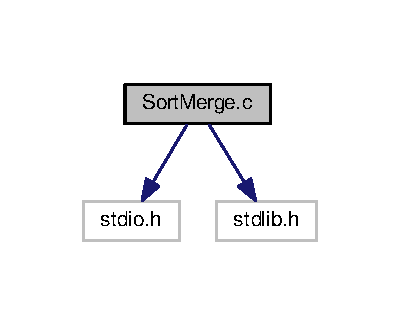
\includegraphics[width=192pt]{SortMerge_8c__incl}
\end{center}
\end{figure}
\subsection*{Classes}
\begin{DoxyCompactItemize}
\item 
struct \hyperlink{structstudent}{student}
\end{DoxyCompactItemize}
\subsection*{Macros}
\begin{DoxyCompactItemize}
\item 
\#define \hyperlink{SortMerge_8c_a70ed59adcb4159ac551058053e649640}{S\+I\+ZE}~10
\item 
\#define \hyperlink{SortMerge_8c_ad79aefee6a8990632311a15e98d9a65f}{N\+A\+M\+E\+S\+I\+ZE}~25
\end{DoxyCompactItemize}
\subsection*{Functions}
\begin{DoxyCompactItemize}
\item 
void \hyperlink{SortMerge_8c_a4905b2143d16f9e71071fb4e408eea73}{write\+Student\+Array} (char filename\mbox{[}$\,$\mbox{]}, \hyperlink{structstudent}{student} a\mbox{[}$\,$\mbox{]}, int n)
\item 
int \hyperlink{SortMerge_8c_adff5ad1d6ceb4e9dcf0f8625a20ee00c}{read\+Student\+Array} (char filename\mbox{[}$\,$\mbox{]}, \hyperlink{structstudent}{student} a\mbox{[}$\,$\mbox{]}, int nmax)
\item 
void \hyperlink{SortMerge_8c_aa9d9fbefcf4d63019ad0f13ca6560227}{sort\+Student\+Array} (\hyperlink{structstudent}{student} table\mbox{[}$\,$\mbox{]}, int n)
\item 
int \hyperlink{SortMerge_8c_a845c5282603a01f1bbbea74e15dd14ae}{merge\+Student\+Array} (\hyperlink{structstudent}{student} table3\mbox{[}$\,$\mbox{]}, \hyperlink{structstudent}{student} table1\mbox{[}$\,$\mbox{]}, int n1, \hyperlink{structstudent}{student} table2\mbox{[}$\,$\mbox{]}, int n2)
\item 
int \hyperlink{SortMerge_8c_a0ddf1224851353fc92bfbff6f499fa97}{main} (int argc, char $\ast$argv\mbox{[}$\,$\mbox{]})
\end{DoxyCompactItemize}


\subsection{Macro Definition Documentation}
\index{Sort\+Merge.\+c@{Sort\+Merge.\+c}!N\+A\+M\+E\+S\+I\+ZE@{N\+A\+M\+E\+S\+I\+ZE}}
\index{N\+A\+M\+E\+S\+I\+ZE@{N\+A\+M\+E\+S\+I\+ZE}!Sort\+Merge.\+c@{Sort\+Merge.\+c}}
\subsubsection[{\texorpdfstring{N\+A\+M\+E\+S\+I\+ZE}{NAMESIZE}}]{\setlength{\rightskip}{0pt plus 5cm}\#define N\+A\+M\+E\+S\+I\+ZE~25}\hypertarget{SortMerge_8c_ad79aefee6a8990632311a15e98d9a65f}{}\label{SortMerge_8c_ad79aefee6a8990632311a15e98d9a65f}
\index{Sort\+Merge.\+c@{Sort\+Merge.\+c}!S\+I\+ZE@{S\+I\+ZE}}
\index{S\+I\+ZE@{S\+I\+ZE}!Sort\+Merge.\+c@{Sort\+Merge.\+c}}
\subsubsection[{\texorpdfstring{S\+I\+ZE}{SIZE}}]{\setlength{\rightskip}{0pt plus 5cm}\#define S\+I\+ZE~10}\hypertarget{SortMerge_8c_a70ed59adcb4159ac551058053e649640}{}\label{SortMerge_8c_a70ed59adcb4159ac551058053e649640}


\subsection{Function Documentation}
\index{Sort\+Merge.\+c@{Sort\+Merge.\+c}!main@{main}}
\index{main@{main}!Sort\+Merge.\+c@{Sort\+Merge.\+c}}
\subsubsection[{\texorpdfstring{main(int argc, char $\ast$argv[])}{main(int argc, char *argv[])}}]{\setlength{\rightskip}{0pt plus 5cm}int main (
\begin{DoxyParamCaption}
\item[{int}]{argc, }
\item[{char $\ast$}]{argv\mbox{[}$\,$\mbox{]}}
\end{DoxyParamCaption}
)}\hypertarget{SortMerge_8c_a0ddf1224851353fc92bfbff6f499fa97}{}\label{SortMerge_8c_a0ddf1224851353fc92bfbff6f499fa97}

\begin{DoxyCode}
99                                 \{
100   \textcolor{keywordtype}{int} n1,     \textcolor{comment}{/* Number of students in first sequence */}
101     n2,       \textcolor{comment}{/* Number of students in second sequence */}
102     n3;       \textcolor{comment}{/* Number of students in resulting sequence */}
103 
104   \hyperlink{structstudent}{student} table1[\hyperlink{SortMerge_8c_a70ed59adcb4159ac551058053e649640}{SIZE}],  \textcolor{comment}{/* Students in first sequence */}
105     table2[\hyperlink{SortMerge_8c_a70ed59adcb4159ac551058053e649640}{SIZE}],        \textcolor{comment}{/* Students in second sequence */}
106     table3[\hyperlink{SortMerge_8c_a70ed59adcb4159ac551058053e649640}{SIZE}+\hyperlink{SortMerge_8c_a70ed59adcb4159ac551058053e649640}{SIZE}];   \textcolor{comment}{/* Students in merged sequence */}
107 
108   \textcolor{keywordflow}{if}(argc!=4)\{
109     printf(\textcolor{stringliteral}{"Usage: %s unsfile1 unsfile2 outfile\(\backslash\)n"}, argv[0]);
110     exit(0);
111   \}
112   n1 = \hyperlink{SortMerge_8c_adff5ad1d6ceb4e9dcf0f8625a20ee00c}{readStudentArray}(argv[1],table1,\hyperlink{SortMerge_8c_a70ed59adcb4159ac551058053e649640}{SIZE});
113   \hyperlink{SortMerge_8c_aa9d9fbefcf4d63019ad0f13ca6560227}{sortStudentArray}(table1,n1);
114   n2 = \hyperlink{SortMerge_8c_adff5ad1d6ceb4e9dcf0f8625a20ee00c}{readStudentArray}(argv[2],table2,\hyperlink{SortMerge_8c_a70ed59adcb4159ac551058053e649640}{SIZE});
115   \hyperlink{SortMerge_8c_aa9d9fbefcf4d63019ad0f13ca6560227}{sortStudentArray}(table2,n2);
116   n3 = \hyperlink{SortMerge_8c_a845c5282603a01f1bbbea74e15dd14ae}{mergeStudentArray}(table3, table1, n1, table2, n2);
117   \hyperlink{SortMerge_8c_a4905b2143d16f9e71071fb4e408eea73}{writeStudentArray}(argv[3],table3,n3);
118 \}
\end{DoxyCode}


Here is the call graph for this function\+:
\nopagebreak
\begin{figure}[H]
\begin{center}
\leavevmode
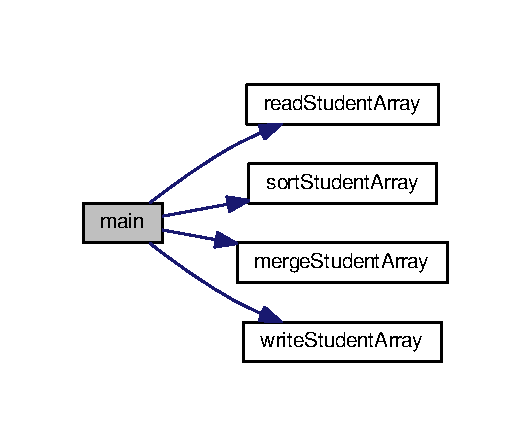
\includegraphics[width=255pt]{SortMerge_8c_a0ddf1224851353fc92bfbff6f499fa97_cgraph}
\end{center}
\end{figure}


\index{Sort\+Merge.\+c@{Sort\+Merge.\+c}!merge\+Student\+Array@{merge\+Student\+Array}}
\index{merge\+Student\+Array@{merge\+Student\+Array}!Sort\+Merge.\+c@{Sort\+Merge.\+c}}
\subsubsection[{\texorpdfstring{merge\+Student\+Array(student table3[], student table1[], int n1, student table2[], int n2)}{mergeStudentArray(student table3[], student table1[], int n1, student table2[], int n2)}}]{\setlength{\rightskip}{0pt plus 5cm}int merge\+Student\+Array (
\begin{DoxyParamCaption}
\item[{{\bf student}}]{table3\mbox{[}$\,$\mbox{]}, }
\item[{{\bf student}}]{table1\mbox{[}$\,$\mbox{]}, }
\item[{int}]{n1, }
\item[{{\bf student}}]{table2\mbox{[}$\,$\mbox{]}, }
\item[{int}]{n2}
\end{DoxyParamCaption}
)}\hypertarget{SortMerge_8c_a845c5282603a01f1bbbea74e15dd14ae}{}\label{SortMerge_8c_a845c5282603a01f1bbbea74e15dd14ae}

\begin{DoxyCode}
81                                    \{
82   \textcolor{comment}{/* It merges into table3 the first n1 student records of table1
}
83 \textcolor{comment}{   * and the first n2 student records of table2. The records in
}
84 \textcolor{comment}{   * table1 and table2 are sorted in nondecreasing order of their 
}
85 \textcolor{comment}{   * name fields. It returns n1+n2.
}
86 \textcolor{comment}{   * WARNING: THIS IS A STUB WHERE WE JUST COPY, NOT MERGE.
}
87 \textcolor{comment}{   */}
88   \textcolor{keywordtype}{int} i,j=0;
89 
90   \textcolor{keywordflow}{for}(i=0;i<n1;i++)\{
91     table3[j++] = table1[i];
92   \}
93   \textcolor{keywordflow}{for}(i=0;i<n2;i++)\{
94     table3[j++] = table2[i];
95   \}
96   \textcolor{keywordflow}{return} n1+n2;
97 \}
\end{DoxyCode}
\index{Sort\+Merge.\+c@{Sort\+Merge.\+c}!read\+Student\+Array@{read\+Student\+Array}}
\index{read\+Student\+Array@{read\+Student\+Array}!Sort\+Merge.\+c@{Sort\+Merge.\+c}}
\subsubsection[{\texorpdfstring{read\+Student\+Array(char filename[], student a[], int nmax)}{readStudentArray(char filename[], student a[], int nmax)}}]{\setlength{\rightskip}{0pt plus 5cm}int read\+Student\+Array (
\begin{DoxyParamCaption}
\item[{char}]{filename\mbox{[}$\,$\mbox{]}, }
\item[{{\bf student}}]{a\mbox{[}$\,$\mbox{]}, }
\item[{int}]{nmax}
\end{DoxyParamCaption}
)}\hypertarget{SortMerge_8c_adff5ad1d6ceb4e9dcf0f8625a20ee00c}{}\label{SortMerge_8c_adff5ad1d6ceb4e9dcf0f8625a20ee00c}

\begin{DoxyCode}
56 \{
57   FILE *fd;  \textcolor{comment}{/* File descriptor used for filename */}
58   \textcolor{keywordtype}{int} i=0;
59   
60   \textcolor{keywordflow}{if}((fd=fopen(filename,\textcolor{stringliteral}{"r"}))==NULL)\{
61     perror(\textcolor{stringliteral}{"fopen"});
62     exit(1);
63   \}
64   \textcolor{keywordflow}{while}(fscanf(fd,\textcolor{stringliteral}{"%s %d %d %d"},
65          a->\hyperlink{structstudent_a4cc31cdf611c0cce37bba9239ea27ae3}{name}, &a->\hyperlink{structstudent_a0044e7dfdd90788897b708b0a64af0ee}{midterm}, &a->\hyperlink{structstudent_a4a15ad9d47eea21ab8b157561f01f2a4}{final}, &a->\hyperlink{structstudent_aa02b98056cfb79a6a5012667be2e717b}{homeworks})!=EOF)\{
66     \textcolor{keywordflow}{if}(++i==nmax)\textcolor{keywordflow}{break};  \textcolor{comment}{/* We have filled up the table */}
67     a++;
68   \}
69   fclose(fd);
70   \textcolor{keywordflow}{return} i;
71 \}
\end{DoxyCode}
\index{Sort\+Merge.\+c@{Sort\+Merge.\+c}!sort\+Student\+Array@{sort\+Student\+Array}}
\index{sort\+Student\+Array@{sort\+Student\+Array}!Sort\+Merge.\+c@{Sort\+Merge.\+c}}
\subsubsection[{\texorpdfstring{sort\+Student\+Array(student table[], int n)}{sortStudentArray(student table[], int n)}}]{\setlength{\rightskip}{0pt plus 5cm}void sort\+Student\+Array (
\begin{DoxyParamCaption}
\item[{{\bf student}}]{table\mbox{[}$\,$\mbox{]}, }
\item[{int}]{n}
\end{DoxyParamCaption}
)}\hypertarget{SortMerge_8c_aa9d9fbefcf4d63019ad0f13ca6560227}{}\label{SortMerge_8c_aa9d9fbefcf4d63019ad0f13ca6560227}

\begin{DoxyCode}
73                                              \{
74   \textcolor{comment}{/* It sorts in nondecreasing order on the basis of their
}
75 \textcolor{comment}{   * names the first n records of table.
}
76 \textcolor{comment}{   * WARNING: THIS IS A NULL STUB.
}
77 \textcolor{comment}{   */}
78 \}
\end{DoxyCode}
\index{Sort\+Merge.\+c@{Sort\+Merge.\+c}!write\+Student\+Array@{write\+Student\+Array}}
\index{write\+Student\+Array@{write\+Student\+Array}!Sort\+Merge.\+c@{Sort\+Merge.\+c}}
\subsubsection[{\texorpdfstring{write\+Student\+Array(char filename[], student a[], int n)}{writeStudentArray(char filename[], student a[], int n)}}]{\setlength{\rightskip}{0pt plus 5cm}void write\+Student\+Array (
\begin{DoxyParamCaption}
\item[{char}]{filename\mbox{[}$\,$\mbox{]}, }
\item[{{\bf student}}]{a\mbox{[}$\,$\mbox{]}, }
\item[{int}]{n}
\end{DoxyParamCaption}
)}\hypertarget{SortMerge_8c_a4905b2143d16f9e71071fb4e408eea73}{}\label{SortMerge_8c_a4905b2143d16f9e71071fb4e408eea73}

\begin{DoxyCode}
32 \{
33   FILE *fd;  \textcolor{comment}{/* File descriptor used for filename */}
34   \textcolor{keywordtype}{int} i;
35   
36   \textcolor{keywordflow}{if}(n<=0)
37     \textcolor{keywordflow}{return};
38   \textcolor{keywordflow}{if}((fd=fopen(filename,\textcolor{stringliteral}{"w"}))==NULL)\{
39     perror(\textcolor{stringliteral}{"fopen"});
40     exit(1);
41   \}
42   \textcolor{keywordflow}{for} (i=0;i<n;i++)\{
43     fprintf(fd,\textcolor{stringliteral}{"%s %d %d %d\(\backslash\)n"},
44       a->\hyperlink{structstudent_a4cc31cdf611c0cce37bba9239ea27ae3}{name}, a->\hyperlink{structstudent_a0044e7dfdd90788897b708b0a64af0ee}{midterm}, a->\hyperlink{structstudent_a4a15ad9d47eea21ab8b157561f01f2a4}{final}, a->\hyperlink{structstudent_aa02b98056cfb79a6a5012667be2e717b}{homeworks});
45     a++;
46   \}
47   fclose(fd);
48 \}
\end{DoxyCode}

%--- End generated contents ---

% Index
\backmatter
\newpage
\phantomsection
\clearemptydoublepage
\addcontentsline{toc}{chapter}{Index}
\printindex

\end{document}
